%% Exemplo de utilizacao do estilo de formatacao normas-utf-tex (http://normas-utf-tex.sourceforge.net)
%% Autores: Hugo Vieira Neto (hvieir@utfpr.edu.br)
%%          Diogo Rosa Kuiaski (diogo.kuiaski@gmail.com)
%% Colaboradores:
%%          Cézar M. Vargas Benitez <cesarvargasb@gmail.com>
%%          Marcos Talau <talau@users.sourceforge.net>


\documentclass[openright]{normas-utf-tex} %openright = o capitulo comeca sempre em paginas impares
%\documentclass[oneside]{normas-utf-tex} %oneside = para dissertacoes com numero de paginas menor que 100 (apenas frente da folha) 

\usepackage[breaklinks=true]{hyperref}
\usepackage[a-3b]{pdfx}   % for PDF/A-3b

\usepackage[alf,abnt-emphasize=bf,bibjustif,recuo=0cm, abnt-etal-cite=3, abnt-etal-list=99]{abntcite} %configuracao correta das referencias bibliograficas.

\usepackage[brazil]{babel} % pacote portugues brasileiro
\usepackage[utf8]{inputenc} % pacote para acentuacao direta
\usepackage[T1]{fontenc} % pacote para  não zicar a acentuação quando copiar o texto do pdf
\usepackage{amsmath,amsfonts,amssymb} % pacote matematico
\usepackage{graphicx} % pacote grafico
%\usepackage{times} % fonte times
\usepackage{quoting}
\usepackage[none]{hyphenat}
\usepackage{microtype}
\usepackage[final]{pdfpages}

%Corrige posicionamento de figuras e tabelas quando não tem texto na página
\makeatletter
\setlength{\@fptop}{0pt}
\makeatother

%Podem utilizar GEOMETRY{...} para realizar pequenos ajustes das margens. Onde, left=esquerda, right=direita, top=superior, bottom=inferior. P.ex.:
%\geometry{left=3.0cm,right=1.5cm,top=4cm,bottom=1cm} 

% ---------- Preambulo ----------
\instituicao{Universidade Tecnológica Federal do Paraná} % nome da instituicao
\programa{Coordenadoria do Curso de Engenharia de Software} % nome do curso
\area{} % Em branco

\documento{Projeto de TCC 1} % [Projeto de TCC 1] ou [Trabalho de Conclusão de Curso] para TCC 2
\nivel{Bacharelado}
\titulacao{Bacharel}

\titulo{\MakeUppercase{Título em Português}} % titulo do trabalho em portugues
\title{Title in English} % titulo do trabalho em ingles

\autor{Nome do Autor} % autor do trabalho
\cita{SOBRENOME, Nome} % sobrenome (maiusculas), nome do autor do trabalho

\palavraschave{Palavra-chave 1, Palavra-chave 2, ...} % palavras-chave do trabalho
\keywords{Keyword 1, Keyword 2, ...} % palavras-chave do trabalho em ingles

\comentario{\UTFPRdocumentodata apresentado como requisito parcial para obtenção do título de \UTFPRtitulacaodata\ em Engenharia de Software da \ABNTinstituicaodata\ (UTFPR).}

\orientador{Prof. Dr. Fulano de Tal} % nome do orientador do trabalho
%\orientador[Orientadora:]{Nome da Orientadora} % <- no caso de orientadora, usar esta sintaxe
\coorientador{Beltrano da Silva} % nome do coorientador do trabalho, caso exista
%\coorientador[Coorientadora:]{Nome da Coorientadora} % <- no caso de coorientadora, usar esta sintaxe
%\coorientador[Coorientadores:]{Nome do Coorientador} % no caso de 2 coorientadores, usar esta sintaxe
%\coorientadorb{Nome do Co-orientador 2}	% este comando inclui o nome do 2o coorientador

\local{Dois Vizinhos} % cidade
\data{\the\year} % ano automatico

%Definir a licença do curso com as seguintes opções (deixar em branco quando não houver):
%by
%by-nc
%by-nc-nd
%by-nc-sa
%by-nd
%by-sa
\licenca{by}

%---------- Inicio do Documento ----------
\begin{document}

\capa % geracao automatica da capa
\folhaderosto % geracao automatica da folha de rosto
%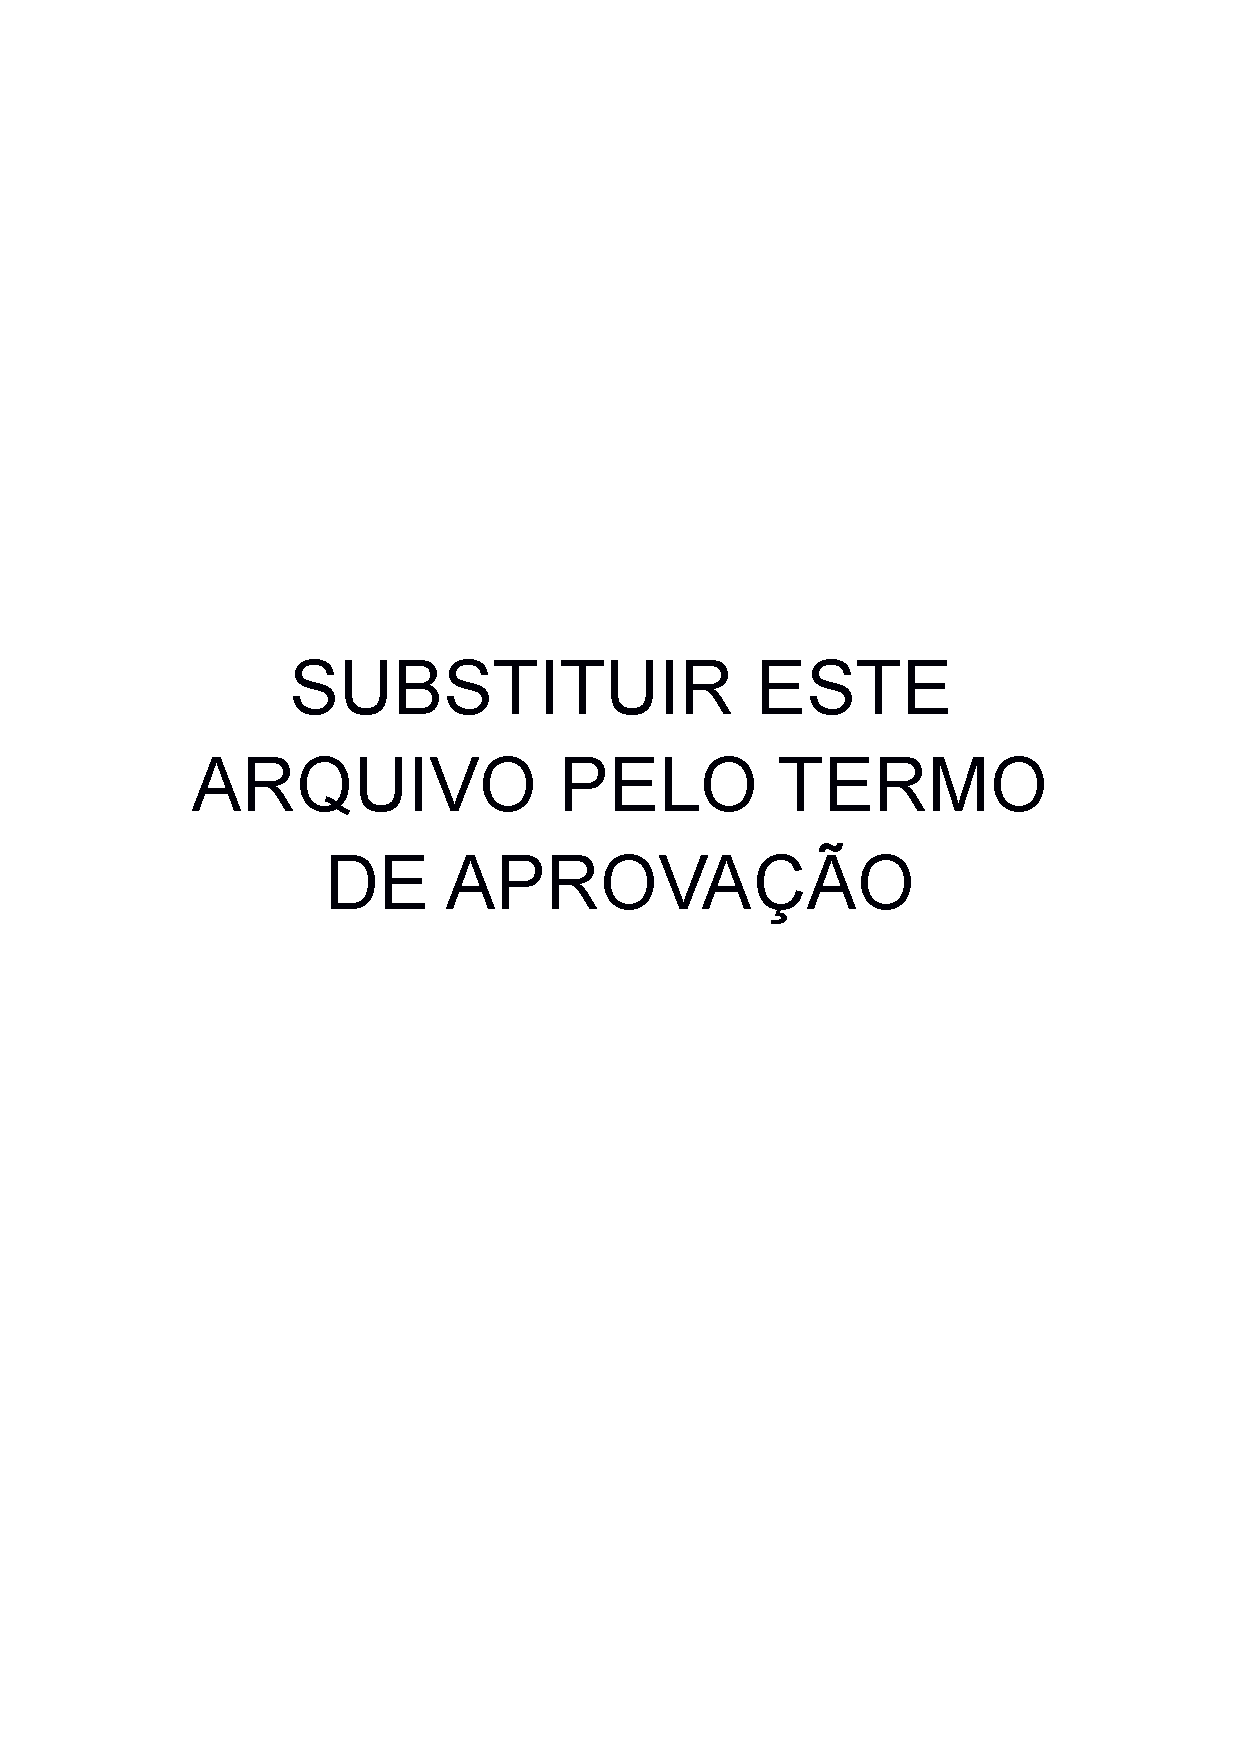
\includepdf{TermoAprovacao.pdf} Termo de Aprovação - o arquivo TermoAprovacao.pdf deve ser substituído pelo fornecido pelo Professor Responsável pelo TCC

% dedicatória (opcional)
\begin{dedicatoria}
A mim mesmo.
\end{dedicatoria}

% agradecimentos (opcional)
\begin{agradecimentos}
Agradeço ao meu querido orientador e a todos os demais que me auxiliaram nesta jornada.
\end{agradecimentos}

% epigrafe (opcional)
\begin{epigrafe}
A vingança nunca é plena, mata a alma e a envenena.

Madruga, Seu.
\end{epigrafe}

%resumo
\begin{resumo}
Elemento obrigatório para TCC 2, constituído de uma sequência de frases concisas e objetivas, fornecendo uma visão rápida e clara do conteúdo do estudo. O texto deverá conter no máximo 500 palavras e ser antecedido pela referência do estudo. Também, não deve conter citações. O resumo deve ser redigido em parágrafo único, espaçamento simples e seguido das palavras representativas do conteúdo do estudo, isto é, palavras-chave, em número de três a cinco, separadas entre si por ponto e finalizadas também por ponto. Usar o verbo na terceira pessoa do singular, com linguagem impessoal (pronome SE), bem como fazer uso, preferencialmente, da voz ativa.
\end{resumo}

%abstract
\begin{abstract}
Elemento obrigatório para o TCC 2. É a versão do resumo em português para o idioma de divulgação internacional. Deve ser antecedido pela referência do estudo. Deve aparecer em folha distinta do resumo em língua portuguesa e seguido das palavras representativas do conteúdo do estudo, isto é, das palavras-chave. Sugere-se a elaboração do resumo (Abstract) e das palavras-chave (Keywords) em inglês; para resumos em outras línguas, que não o inglês, consultar o departamento / curso de origem.
\end{abstract}

% listas (opcionais, mas recomenda-se a partir de 5 elementos)
\listadefiguras % geracao automatica da lista de figuras
\listadetabelas % geracao automatica da lista de tabelas
\listadequadros % geracao automatica da lista de quadros
\listadesiglas % geracao automatica da lista de siglas
\listadesimbolos % geracao automatica da lista de simbolos

% sumario
\sumario % geracao automatica do sumario


%---------- Inicio do Texto ----------
% recomenda-se a escrita de cada capitulo em um arquivo texto separado (exemplo: intro.tex, fund.tex, exper.tex, concl.tex, etc.) e a posterior inclusao dos mesmos no mestre do documento utilizando o comando \include{}, da seguinte forma:

\chapter{Introdução}

A introdução de um relatório técnico de conclusão de curso constitui uma seção primordial que estabelece o contexto do projeto. Ela deve iniciar com uma exposição clara do tema central do trabalho, abordando a relevância do assunto dentro do campo da pesquisa proposta. Subsequentemente, é imprescindível delimitar o escopo do projeto, especificando os limites e o foco da pesquisa ou desenvolvimento realizado \cite{abnTeX2009}.
Os objetivos do projeto devem ser claramente delineados na introdução, fornecendo uma visão geral das metas que o trabalho almeja alcançar. Esses objetivos podem ser subdivididos em geral e específicos, se necessário, para uma compreensão mais detalhada das intenções do projeto. Detalhes sobre a metodologia empregada, os resultados e as conclusões não devem ser abordados nesta seção, pois serão tratados em partes específicas do relatório.
Ademais, a introdução pode incluir uma breve revisão da literatura relacionada ao tema, destacando trabalhos anteriores que tenham contribuído para a fundamentação teórica do projeto. Esse passo é importante pois auxilia na demonstração da base científica sobre a qual o trabalho, ainda que técnico, está construído e na justificativa da importância da pesquisa realizada.
Por fim, a introdução deve ser redigida de forma concisa e objetiva, visando capturar o interesse do leitor e fornecer uma visão geral clara do trabalho realizado. Ela serve como um prelúdio para as seções subsequentes que detalharão o projeto em profundidade.


\section{Objetivo Geral}

Indicar o objetivo geral.

\section{Objetivos Específicos}

Indicar cada objetivo específico do trabalho.

\section{Descrição da regra de negócio}

A descrição da regras de negocio é uma parte crucial do TCC, visto que elas definem como uma ferramenta ou produto de software deve operar para atender às necessidades dos usuários e às normas da organização. Uma descrição clara e detalhada garante que todos os stakeholders compreendam os requisitos e funcionalidades do software.


\section{Justificativa/Contextualização}

Esta subseção serve para explicar a importância e a relevância do projeto a ser realizado. Ela deve fornecer argumentos que demonstrem a necessidade do estudo, destacando o impacto potencial dos resultados na área de conhecimento ou na prática profissional. Essa subseção também contextualiza o problema abordado, situando-o em um quadro mais amplo, como tendências atuais, desafios específicos do setor ou lacunas na literatura existente. Ao justificar o trabalho, o autor estabelece a base para a compreensão do leitor sobre a importância do projeto e sua contribuição para a área de estudo ou aplicação prática.
\chapter{Desenvolvimento}

A seção de desenvolvimento de um relatório técnico é a parte central do documento, onde são detalhadas as atividades a serem realizadas e os métodos inicialmente planejados para serem empregados. Esta seção é dividida em subseções que podem variar de acordo com a natureza do projeto. 
Nesta parte do documento, é esperado que o autor faça uso dos conhecimentos de Engenharia de Software e áreas afins para estabelecer as bases do projeto a ser elaborado. Informações como regras de negócios, domínio da aplicação, metodologias e métodos de desenvolvimento, requisitos e funcionalidades, persistência de dados são apenas algumas das informações que poderão ser necessárias a depender do projeto proposto.  Em geral, algumas seções a serem incluídas são: 

\begin{itemize}
    \item Metodologia: Descrição detalhada das técnicas e processos que devem ser utilizados no desenvolvimento do projeto, incluindo ferramentas, linguagens de programação, frameworks e metodologias de desenvolvimento de software. Indicar quais são os principais fundamentos (algoritmos, paradigmas, teorias) a serem empregados. Cada fundamento utilizado deve ser justificado. Indicar também quais são as principais tecnologias (ambientes de desenvolvimento, linguagens de programação, plataformas de hardware) a serem empregadas. Cada tecnologia utilizada deve ser justificada. 

    \item Implementação: Detalhamento da construção do sistema ou aplicação, abordando aspectos como arquitetura de software, módulos desenvolvidos, funcionalidades implementadas e interfaces de usuário.

    \item Testes: Apresentação das estratégias de teste que serão adotadas, incluindo testes unitários, de integração, de sistema e de aceitação.

    \item Resultados esperados: Exposição dos resultados a serem alcançados com o desenvolvimento do projeto, podendo incluir métricas de desempenho, feedback dos usuários, impacto nos processos ou práticas existentes e contribuições para a área de conhecimento.
\end{itemize}


Para organizar todas estas informações, o autor precisará fazer uso de seções e subseções. As explicações sobre como proceder com a formatação destes recursos são apresentadas a seguir.

\section{Funcionalidades}

Descreva nesta seção as funcionalidades que a ferramenta ou produto de software terá após seu desenvolvimento. Cada funcionalidade deve ser explicada de forma clara e completa, de modo que qualquer leitor possa entender exatamente o que o software faz e como ele atende às necessidades identificadas na seção de descrição da regra de negócio.
Sugere-se que as funcionalidades da ferramenta ou produto de software sejam apresentadas de forma organizada, agrupando-as por módulos e categorias, se aplicável. Por exemplo, se o software tem um módulo de administração e um módulo de usuário, agrupe as funcionalidades de acordo. A seguir é apresentada uma sugestão de itens a serem abordados para cada funcionalidade, ficando claro que é só uma sugestão e que o orientador deverá ser consultado a respeito.

\subsection{Funcionalidade 1}
\begin{itemize}
    \item \textbf{Nome da Funcionalidade}: Dê um nome claro e descritivo.
    \item \textbf{Objetivo}: Explique o propósito da funcionalidade e o problema específico que ela resolve.
    \item \textbf{Descrição}: Detalhe como a funcionalidade funciona, incluindo fluxos de trabalho, interações com o usuário e exemplos práticos de uso.
    \item \textbf{Requisitos}: Liste os requisitos necessários para a funcionalidade, como dados de entrada, pré-condições e pós-condições.
    \item \textbf{Interfaces}: Descreva a interface do usuário relacionada à funcionalidade, se aplicável, incluindo capturas de tela, wireframes ou protótipos.
    \item \textbf{Exemplo de Uso}: Forneça um exemplo concreto de como a funcionalidade é utilizada na prática, idealmente com um cenário realista ou um caso de uso.
\end{itemize}

\section{Persistência de dados}

Na Seção de "Persistência de Dados", os estudantes devem explicar como os dados são armazenados, gerenciados e recuperados pelo software. Isso inclui a descrição da estrutura do banco de dados, o modelo de dados adotado, as tecnologias utilizadas, e exemplos de consultas e operações realizadas sobre os dados. 
Sugere-se que sejam apresentadas todas as estruturas e modelos que são necessários para compreensão da persistência dos dados na ferramenta ou produto de software a ser desenvolvido, como Diagramas ER, esquemas de tabelas e fluxogramas. Além disso, a inclusão de detalhes técnicos específicos, como tipos de dados, restrições de integridade e exemplos de consultas SQL é importante para melhor compreensão. 


\section{Tecnologias Utilizadas}
% SEÇÃO ORIBRIGATÓRIA PARA TCC 2 E OPCIONAL PARA O TCC 1 

Nesta seção, os estudantes devem listar e descrever as principais tecnologias utilizadas no desenvolvimento do software. Isso inclui linguagens de programação, frameworks, bibliotecas, ferramentas de desenvolvimento, plataformas e serviços externos. A explicação deve detalhar o papel de cada tecnologia e justificar sua escolha.
Se possível, detalhe as versões específicas das tecnologias usadas e explique qualquer configuração ou customização realizada, e explique como cada tecnologia suportou a implementação das funcionalidades descritas anteriormente. 

\section{Avaliação/Testes}
% SEÇÃO ORIBRIGATÓRIA PARA TCC 2 E OPCIONAL PARA O TCC 1 

Esta seção é dedicada a descrição do processo de avaliação e testes realizados no software. Isso inclui os tipos de testes aplicados, as ferramentas utilizadas, os resultados obtidos e como esses resultados foram usados para melhorar o sistema.

\section{Cronograma}
% SEÇÃO ORIBRIGATÓRIA PARA TCC 1. 
% DEVE SER REMOVIDA PARA O TCC 2

A subseção Cronograma de um relatório técnico é fundamental para organizar e planejar as etapas do projeto ao longo do tempo. Geralmente apresentado em forma de tabela ou gráfico de Gantt, o cronograma lista as atividades, suas datas de início e término previstas, e a duração. Isso ajuda a visualizar a sequência das tarefas, identificar períodos críticos e monitorar o andamento do projeto. É uma ferramenta essencial para garantir que o trabalho seja concluído dentro do prazo estipulado.
Devem estar detalhadas, de forma lógica, linear e cronológica, todas as etapas do projeto que esclareçam como o produto será gerado. 

\section{Como utilizar figuras}

São ilustrações: figuras, quadros, gráficos, fotografias, retratos, desenhos, gravuras, imagens, fluxogramas, organogramas, esquemas, mapas, plantas e diferenciam-se das tabelas. As ilustrações devem ser inseridas o mais próximo possível do texto a que se refere.
Qualquer que seja o tipo de ilustração, sua identificação aparece na parte inferior, precedida da palavra designativa, seguida de seu número de ordem de ocorrência no texto, em algarismos arábicos, do respectivo título e/ou legenda. A fonte deve ser tamanho 10 e em negrito. Após a legenda, deve-se citar a fonte de onde foi retirada a ilustração, precedida da palavra “Fonte” (Autor, data), bem como, deve-se referenciá-la, de forma completa, na seção Referências.

Na Figura~\ref{fig:dummy} \'e apresentado um exemplo de gr\'afico flutuante. Esta figura aparece automaticamente na lista de figuras. Para uso avan\c{c}ado de gr\'aficos no \LaTeX, recomenda-se a consulta de literatura especializada~\cite{Goossens2007}.


\begin{figure}[!htb]
	\centering
	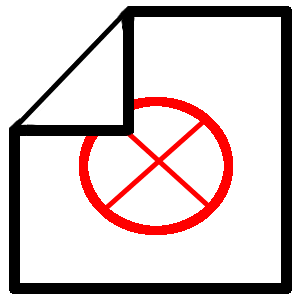
\includegraphics[width=0.2\textwidth]{Imagens/dummy.png} % <- formatos PNG, JPG e PDF
	\caption[Exemplo de uma figura]{Exemplo de uma figura onde aparece uma imagem sem nenhum significado especial.}
	\fonte{\cite{abnTeX2009}}
	\label{fig:dummy}
\end{figure}


\section{Como utilizar tabelas}

Uma tabela deve apresentar dados numéricos de modo resumido e é utilizada principalmente para a apresentação de comparações. Deve-se seguir tal padrão em todo o trabalho, constando também na lista de tabelas, separada da lista de ilustrações. Os quadros não devem ser chamados de tabelas, uma vez que se diferenciam destas por apresentarem as laterais fechadas e o conteúdo não numérico\footnote{Para as regras gerais de apresentação de tabelas, ver página 61 das Normas para Elaboração de Trabalhos Acadêmicos da UTFPR, dispon\'ivel em: http://www.utfpr.edu.br/documentos/normas\_trabalhos\_utfpr.pdf}.

Tamb\'em \'e apresentado o exemplo da tabela~\ref{tab:correlacao}, que aparece automaticamente na lista de tabelas. Informa\c{c}\~oes sobre a constru\c{c}\~ao de tabelas no \LaTeX\ podem ser encontradas na literatura especializada~\cite{Lamport1986,Buerger1989,Kopka2003,Mittelbach2004}.

\begin{table}[!htb]
	\centering
	\caption[Exemplo de uma tabela]{Exemplo de uma tabela mostrando a correla\c{c}\~ao entre x e y.}
	\label{tab:correlacao}
	\begin{tabular}{cc}
		\hline 
		x & y \\
		\hline
		1 & 2 \\
		3 & 4 \\
		5 & 6 \\
		7 & 8 \\
		\hline 
	\end{tabular}
	\fonte{Autoria pr\'opria.}
\end{table}

\section{Como utilizar equações}

A transformada de Laplace \'e dada na equa\c{c}\~ao~(\ref{eq:laplace}), enquanto a equa\c{c}\~ao~(\ref{eq:dft}) apresenta a formula\c{c}\~ao da transformada discreta de Fourier bidimensional\footnote{Deve-se reparar na formata\c{c}\~ao esteticamente perfeita destas equa\c{c}\~oes!}.

\begin{equation}
X(s) = \int\limits_{t = -\infty}^{\infty} x(t) \, \text{e}^{-st} \, dt
\label{eq:laplace}
\end{equation}

\begin{equation}
F(u, v) = \sum_{m = 0}^{M - 1} \sum_{n = 0}^{N - 1} f(m, n) \exp \left[ -j 2 \pi \left( \frac{u m}{M} + \frac{v n}{N} \right) \right]
\label{eq:dft}
\end{equation}

\section{Como utilizar siglas e símbolos}

O pacote \textsc{abn}\TeX\ permite ainda a defini\c{c}\~ao de siglas e s\'imbolos com indexa\c{c}\~ao autom\'atica atrav\'es dos comandos {\ttfamily \textbackslash sigla\{\}\{\}} e {\ttfamily \textbackslash simbolo\{\}\{\}}. Por exemplo, o significado das siglas\sigla{CPGEI}{Programa de P\'os-gradua\c{c}\~ao em Engenharia El\'etrica e Inform\'atica Industrial},\sigla{DAELN}{Departamento Acad\^emico de Eletr\^onica} e\sigla{UTFPR}{Universidade Tecnol\'ogica Federal do Paran\'a} aparecem automaticamente na lista de siglas, bem como o significado dos s\'imbolos\simbolo{$\lambda$}{comprimento de onda},\simbolo{$v$}{velocidade} e\simbolo{$f$}{frequ\^encia} aparecem automaticamente na lista de s\'imbolos. Mais detalhes sobre o uso destes e outros comandos do \textsc{abn}\TeX\ s\~ao encontrados na sua documenta\c{c}\~ao espec\'ifica~\cite{abnTeX2009}.


\section{Seção Secundária}

\subsection{Seção Terciária}

Seção terciária \cite{Lamport1986, Kopka2003}

\subsubsection[Seção quaternária]{\underline{Seção quaternária}}

Seção quaternária.
% \chapter{Recursos}

Apresente aqui todos os recursos essenciais ao desenvolvimento do projeto. O(s) aluno(s) deve(m) mencionar também a origem dos recursos (próprios, externos ou da UTFPR) e a viabilidade do projeto.

Devem ser apresentados aqui os recursos de software, incluindo os principais fundamentos (teorias, algoritmos, paradigmas) e tecnologias (ambientes de desenvolvimento, linguagens de programação) a serem empregados. Especifique a origem dos recursos de software. % Não obrigatório porém, a critério do estudante/orientador pode ser adicionado
% \chapter{Resultados}

Resultados finais do trabalho. % Não obrigatório porém, a critério do estudante/orientador pode ser adicionado
\chapter{Conclusões}

As conclusões do trabalho devem ser expostas de maneira clara, lógica e concisa. Fale das dificuldades e facilidades encontradas durante a execução da proposta até o momento.


%---------- Referencias ----------
\clearpage % this is need for add +1 to pageref of bibstart used in 'ficha catalografica'.
\label{bibstart}
\bibliography{reflatex} % geracao automatica das referencias a partir do arquivo reflatex.bib
\label{bibend}


%---------- Apendices (opcionais) ----------
\apendice

\chapter{Título do Apêndice}

Elemento opcional, que consiste em texto ou documento elaborado pelo autor, a fim de complementar sua argumentação, sem prejuízo da unidade nuclear do trabalho.

Os apêndices devem ser identificados por letras maiúsculas consecutivas, seguidas de travessão e respectivo título.


% ---------- Anexos (opcionais) ----------
\anexo

\chapter{Título do Anexo}

Elemento opcional, que consiste em texto ou documento não elaborado pelo autor, que serve de fundamentação, comprovação e ilustração.

Os anexos devem ser identificados por letras maiúsculas consecutivas, seguidas de travessão e respectivo título.


% --------- Lista de siglas --------
%\textbf{* Observa\c{c}\~oes:} a lista de siglas nao realiza a ordenacao das siglas em ordem alfabetica
% Em breve isso sera implementado, enquanto isso:
%\textbf{Sugest\~ao:} crie outro arquivo .tex para siglas e utilize o comando \sigla{sigla}{descri\c{c}\~ao}.
%Para incluir este arquivo no final do arquivo, utilize o comando \input{arquivo.tex}.
%Assim, Todas as siglas serao geradas na ultima pagina. Entao, devera excluir a ultima pagina da versao final do arquivo
% PDF do seu documento.


%-------- Citacoes ---------
% - Utilize o comando \citeonline{...} para citacoes com o seguinte formato: Autor et al. (2011).
% Este tipo de formato eh utilizado no comeco do paragrafo. P.ex.: \citeonline{autor2011}

% - Utilize o comando \cite{...} para citacoeses no meio ou final do paragrafo. P.ex.: \cite{autor2011}



%-------- Titulos com nomes cientificos (titulo, capitulos e secoes) ----------
% Regra para escrita de nomes cientificos:
% Os nomes devem ser escritos em italico, 
%a primeira letra do primeiro nome deve ser em maiusculo e o restante em minusculo (inclusive a primeira letra do segundo nome).
% VEJA os exemplos abaixo.
% 
% 1) voce nao quer que a secao fique com uppercase (caixa alta) automaticamente:
%\section[nouppercase]{\MakeUppercase{Estudo dos efeitos da radiacao ultravioleta C e TFD em celulas de} {\textit{Saccharomyces boulardii}}
%
% 2) por padrao os cases (maiusculas/minuscula) sao ajustados automaticamente, voce nao precisa usar makeuppercase e afins.
% \section{Introducao} % a introducao sera posta no texto como INTRODUCAO, automaticamente, como a norma indica.


\end{document}